\documentclass[a4paper]{article}
\usepackage[utf8]{inputenc}
\usepackage[russian]{babel}
\usepackage[T2]{fontenc}
\usepackage[warn]{mathtext}
\usepackage{graphicx}
\usepackage{amsmath}
\usepackage{floatflt}
\usepackage[left=20mm, top=20mm, right=20mm, bottom=20mm, footskip=10mm]{geometry}


\graphicspath{ {images/} }
\usepackage{multicol}
\setlength{\columnsep}{2cm}


\begin{document}

\begin{titlepage}
	\centering
	\vspace{5cm}
	{\scshape\LARGE Московский физико-технический институт \par}
	\vspace{4cm}
	{\scshape\Large Лабораторная работа \par}
	\vspace{1cm}
	{\huge\bfseries Опыт Франка-Герца \par}
	\vspace{1cm}
	\vfill
\begin{flushright}
	{\large выполнила студентка 653 группы ФФКЭ}\par
	\vspace{0.3cm}
	{\LARGE Карпова Татьяна} \par

\end{flushright}
	

	\vfill

% Bottom of the page
	Долгопрудный, 2018 г.
\end{titlepage}

\section{Цель работы}
Методом электронного возбуждения измерить энергию первого уровня атома гелия в динамическом и статическом режимах

\section{В работе используюются:}
\begin{itemize}
    \item трёхэлектродная лампа ЛМ-2
    \item батарея 4,5 В
    \item микроамперметр
    \item понижающий трансформатор
    \item осциллограф
    \item блок источников питания
    \item вольтметр В7-22А
\end{itemize}

\section{Теоретические положения}
Опыт Франка-Герца подтверждает существование дискретных уровней энергии атомов. Разреженный одноатомный газ заполняет трёхэлектродную лампу. Электроны, испускаемые разогретым катодом, ускоряются в постоянном электрическом поле, созданном между катодом и сетчатым анодом лампы. Передвигаясь от катода к аноду, электроны сталкиваются с атомами гелия.
\begin{itemize}
    \item энергия электрона недостаточна, чтобы возбудить/ионизировать атом -> \textit{упругое столкновение}, электрон не теряет энергию
    \item при большой разности потенциалов энергия электрона достаточна для возбуждения атомов -> \textit{неупругое столкновение}, кинетическая энергия передаётся одному из атомных электронов, в результате чего происходит:
    \begin{itemize}
        \item \textbf{возбуждение} - переход одного из атомных электронов на свободный энергетический уровень
        \item \textbf{ионизация} - отрыв электрона от атома 
    \end{itemize}
\end{itemize}

\begin{figure}[h]
\begin{center}
\begin{minipage}[h]{0.45\linewidth}
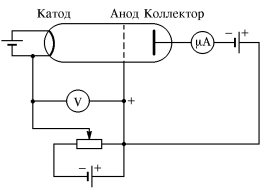
\includegraphics[width=1\linewidth]{fig1.PNG}
\caption{Схема опыта Франка и Герца} %% подпись к рисунку
\label{ris:experimoriginal} %% метка рисунка для ссылки на него
\end{minipage}
\hfill 
\begin{minipage}[h]{0.45\linewidth}
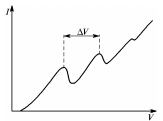
\includegraphics[width=1\linewidth]{fig2.PNG}
\caption{Схематический вид зависимости тока коллектора от напряжения на аноде}
\label{ris:experimcoded}
\end{minipage}
\end{center}
\end{figure}

Объясним вид зависимости тока коллектора (измеряется микроамперметром) от напряжения на аноде. При увеличении потенциала анода ток в лампе сначала растёт (зависимость, подобная ВАХ вакуумного диода). Когда энергия электронов становится достаточной для возбуждения атомов, ток коллектора резко уменьшается. Это происходит потому, что при неупругих соударениях с атомами электроны теряют свою энергию и не могут преодолеть задерживающее напряжение (около 1 В) между анодом и коллектором. При дальнейшем увеличении потенциала ток коллектора вновь возрастает: электроны, испытавшие неупругие соударения, при дальнейшем движении к аноду успевают набрать энергию, достаточную для преодоления задерживающего потенциала. Следующее замедление роста тока происходит в момент, когда часть электронов неупруго сталкивается с атомами два раза. Таким образом, на кривой зависимости тока коллектора от напряжения анода имеется ряд максимумов и минимумов, отстоящих друг от друга на равные расстояния, равные энергии первого возбуждённого состояния.

\section{Экспериментальная установка}

\begin{figure}[h]
    \centering
    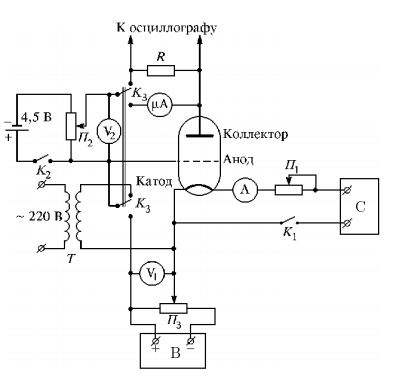
\includegraphics[width=12cm]{fig3.PNG}
    \caption{Схема экспериментальной установки}
    \label{fig:vac}
\end{figure}

На рис.3 обозначены:
\begin{itemize}
    \item А - амперметр
    \item Б7-4 - стабилизированный источник питания (подаёт напряжение накала)
    \item $K_1$ - тумблер для включения в цепь источника Б7-4
    \item Б5-10 - выпрямитель (подаёт на анод ускоряющее напряжение)
    \item $Pi_3$ - потенциометр, регулирующий величину ускоряющего напряжения
    \item $V_1$ - вольтметр, измеряющий величину ускоряющего напряжения
    \item 4,5 В - батарея КБСЛ - источник задерживающего потенциала
    \item $Pi_2$ - потенциометр, регулирующий величину задерживающего потенциала
    \item $V_2$ - вольтметр, измеряющий величину задерживающего потенциала
    \item $\mu A$ - микроамперметр - регистрирует ток в цепи коллектора
    \item $K_3$ - ключ, переключающий схему из статического режима в динамический
    \item Т - понижающий трансформатор - подаёт ускоряющий потенциал при динамическом режиме
    \item - нагрузочный резистор
\end{itemize}

\section{Выполнение работы}
\subsection{Получение вольт-амперной характеристики $I_k = f(V_a)$ на экране осциллографа С1-38 (динамический метод)}
\begin{enumerate}
    \item Подготовим приборы к работе, поставим переключатель режима в положение "Динамич."
    \item Добьёмся с помощью регуляторов на осциллографе чёткой картины на экране
    \item При максимальном ускоряющем напряжении измерим на экране расстояние между максимумами и между минимумами осциллограммы. Измерения проведём при трёх значениях задерживающего напряжения: 4, 6 и 8 В. Результаты измерений занесём в таблицу 1. Фотографии полученных осциллограмм приведём на рисунках 4-6.
 
\begin{table}[h]
    \centering
    \begin{center}
    \caption{Максимумы и минимумы напряжения на осциллограммах}
    \end{center}
    \vspace{0.1cm}
    \label{tab:my_label}
    \begin{tabular}{ |p{3.5cm}||p{1cm}|p{1cm}|p{1cm}|p{1cm}|p{2.5cm}|p{1cm}|p{1cm}|}
 \hline
Задерж. напряжение & $V_{max_1}$ & $V_{max_2}$ & $V_{min_1}$ & $V_{min_2}$ & Погрешность & \triangle V_{max} & \triangle V_{min}\\
 \hline
 4 В & 0 В & 13 В & 2 В & 19 В & 1 В & 13 В & 17 В\\
\hline
 6 В & -4 В & 10 В & 0 В & 17,5 В & 1 В & 14 В & 17,5 В\\
\hline
 8 В & -4 В & 10 В & 0 В & 18 В & 2 В & 14 В & 18 В\\
\hline

\end{tabular}
\end{table} 
    
\begin{figure}[h]
\begin{center}
\begin{minipage}[h]{0.45\linewidth}
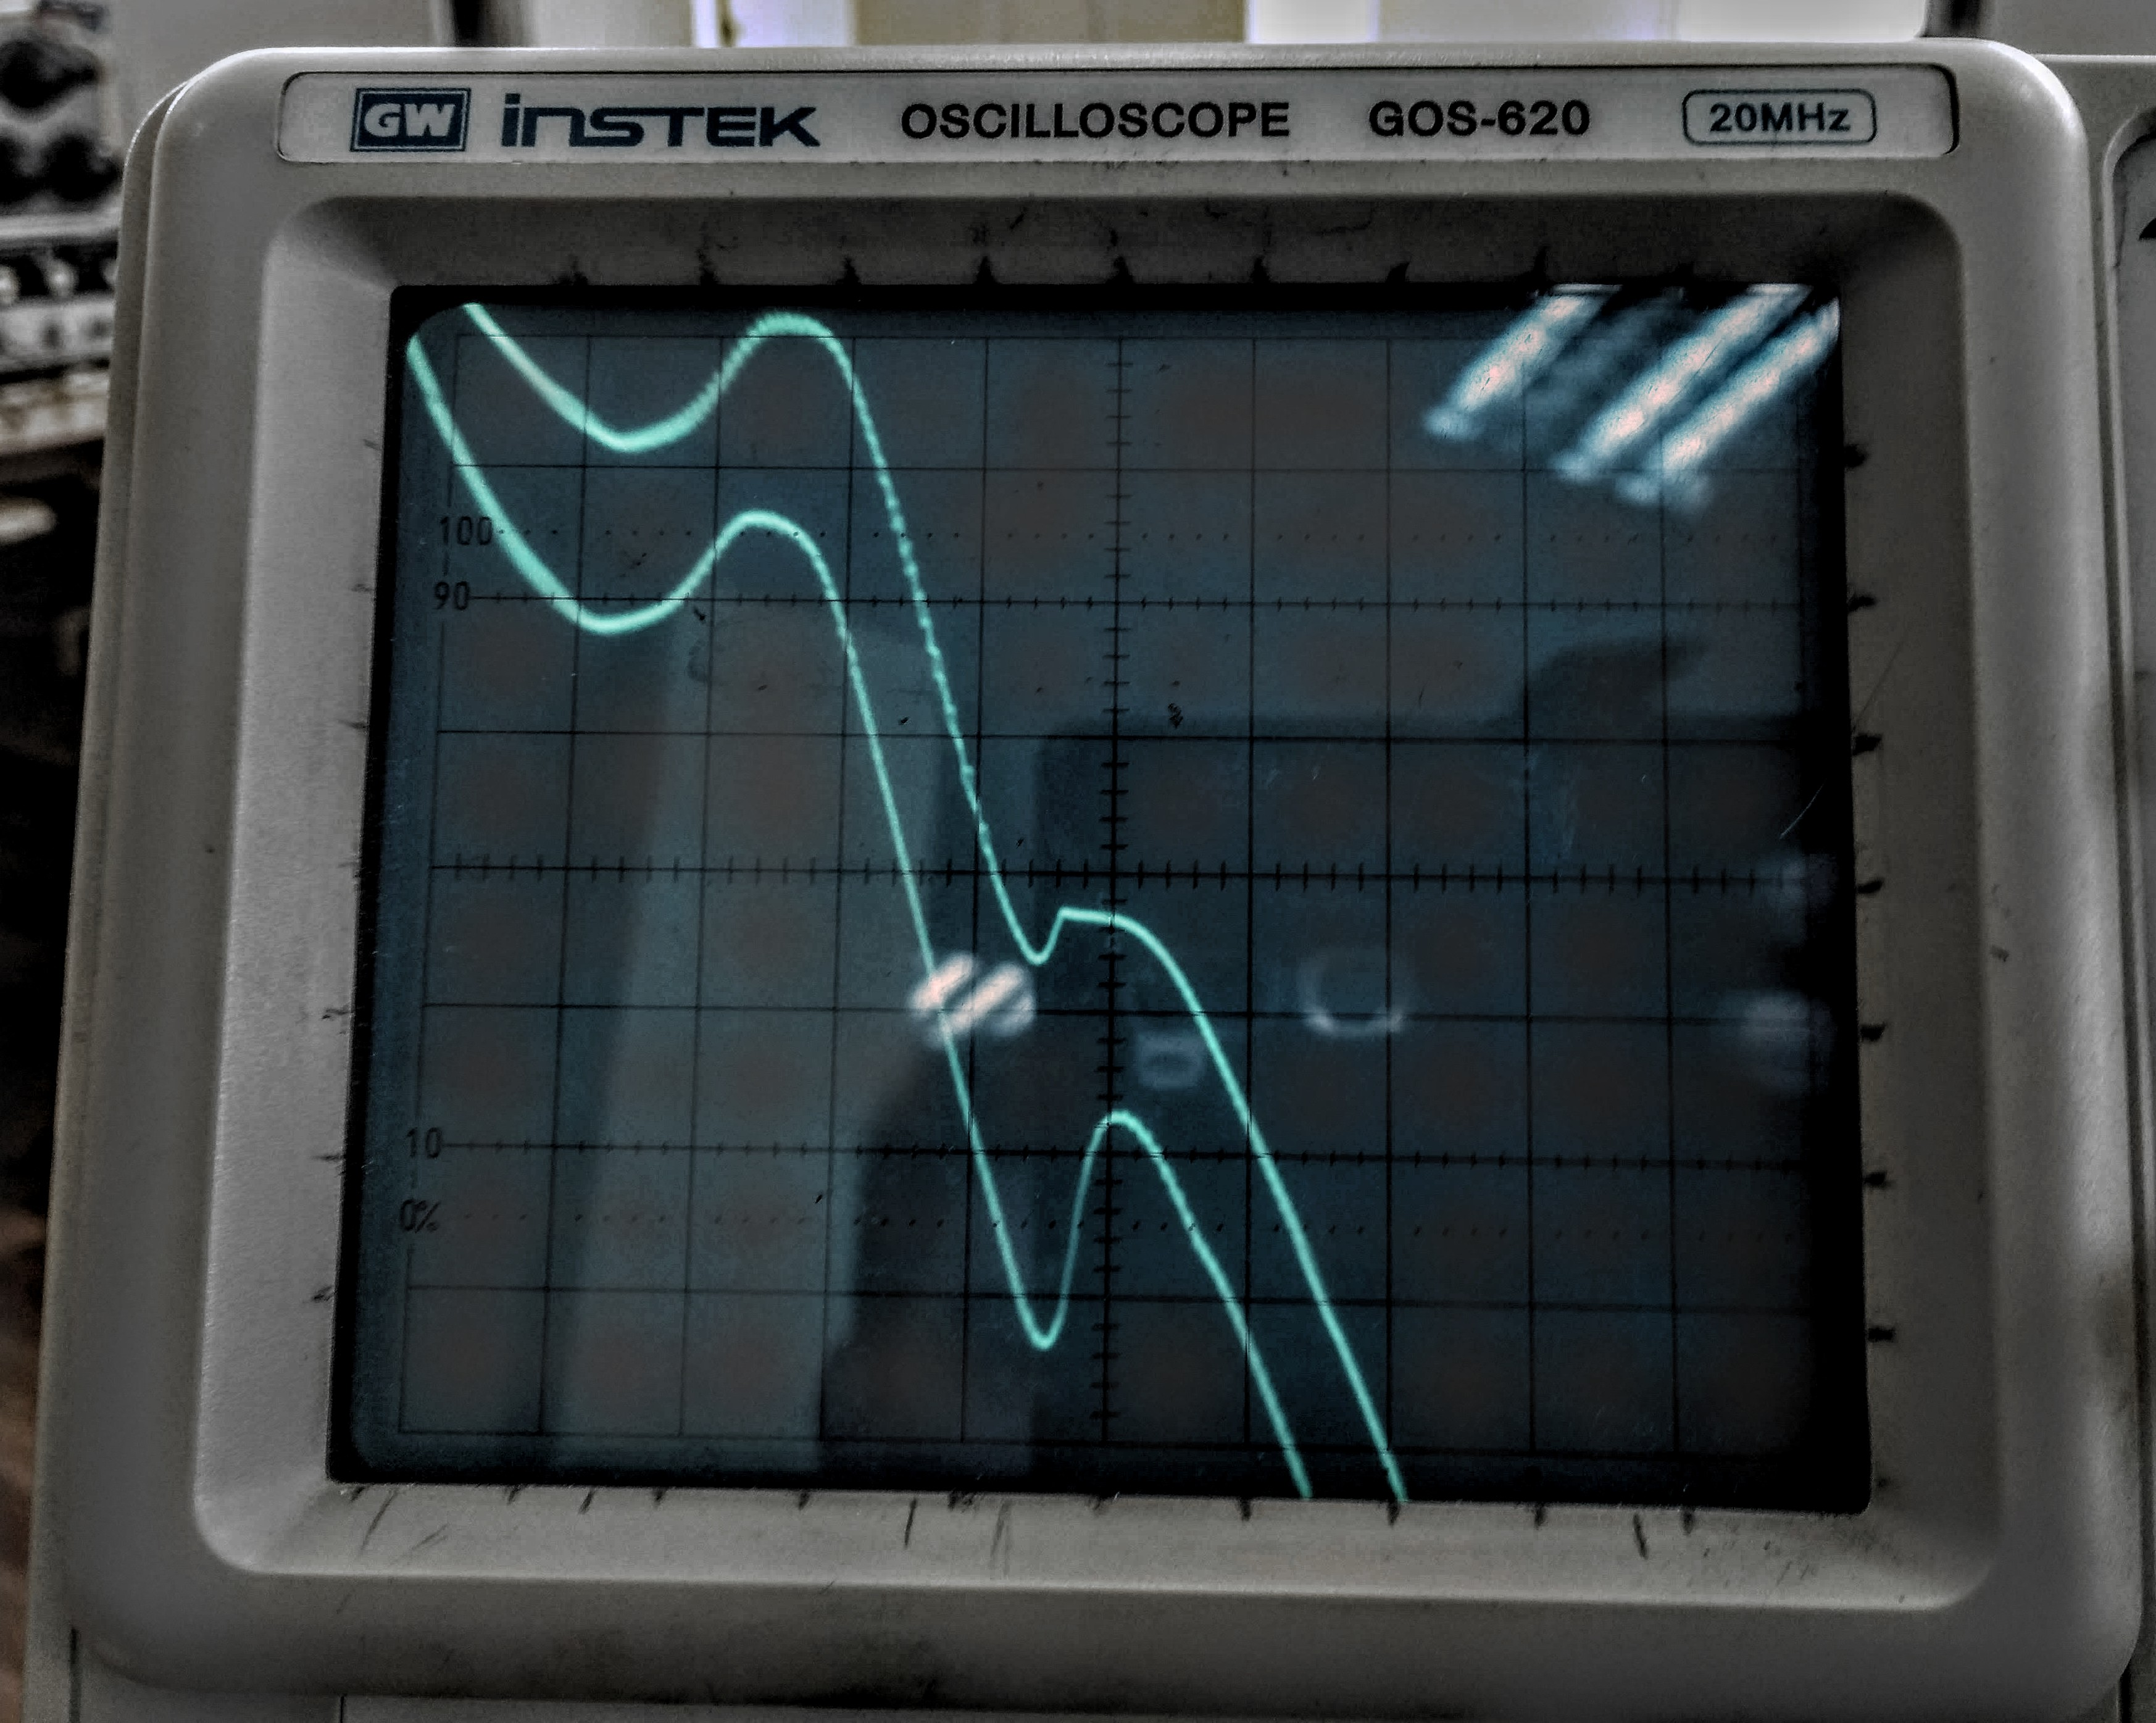
\includegraphics[width=1\linewidth]{4_V.jpg}
\caption{Осциллограмма при задерживающем напряжении 4 В} %% подпись к рисунку
\label{ris:experimoriginal} %% метка рисунка для ссылки на него
\end{minipage}
\hfill 
\begin{minipage}[h]{0.45\linewidth}
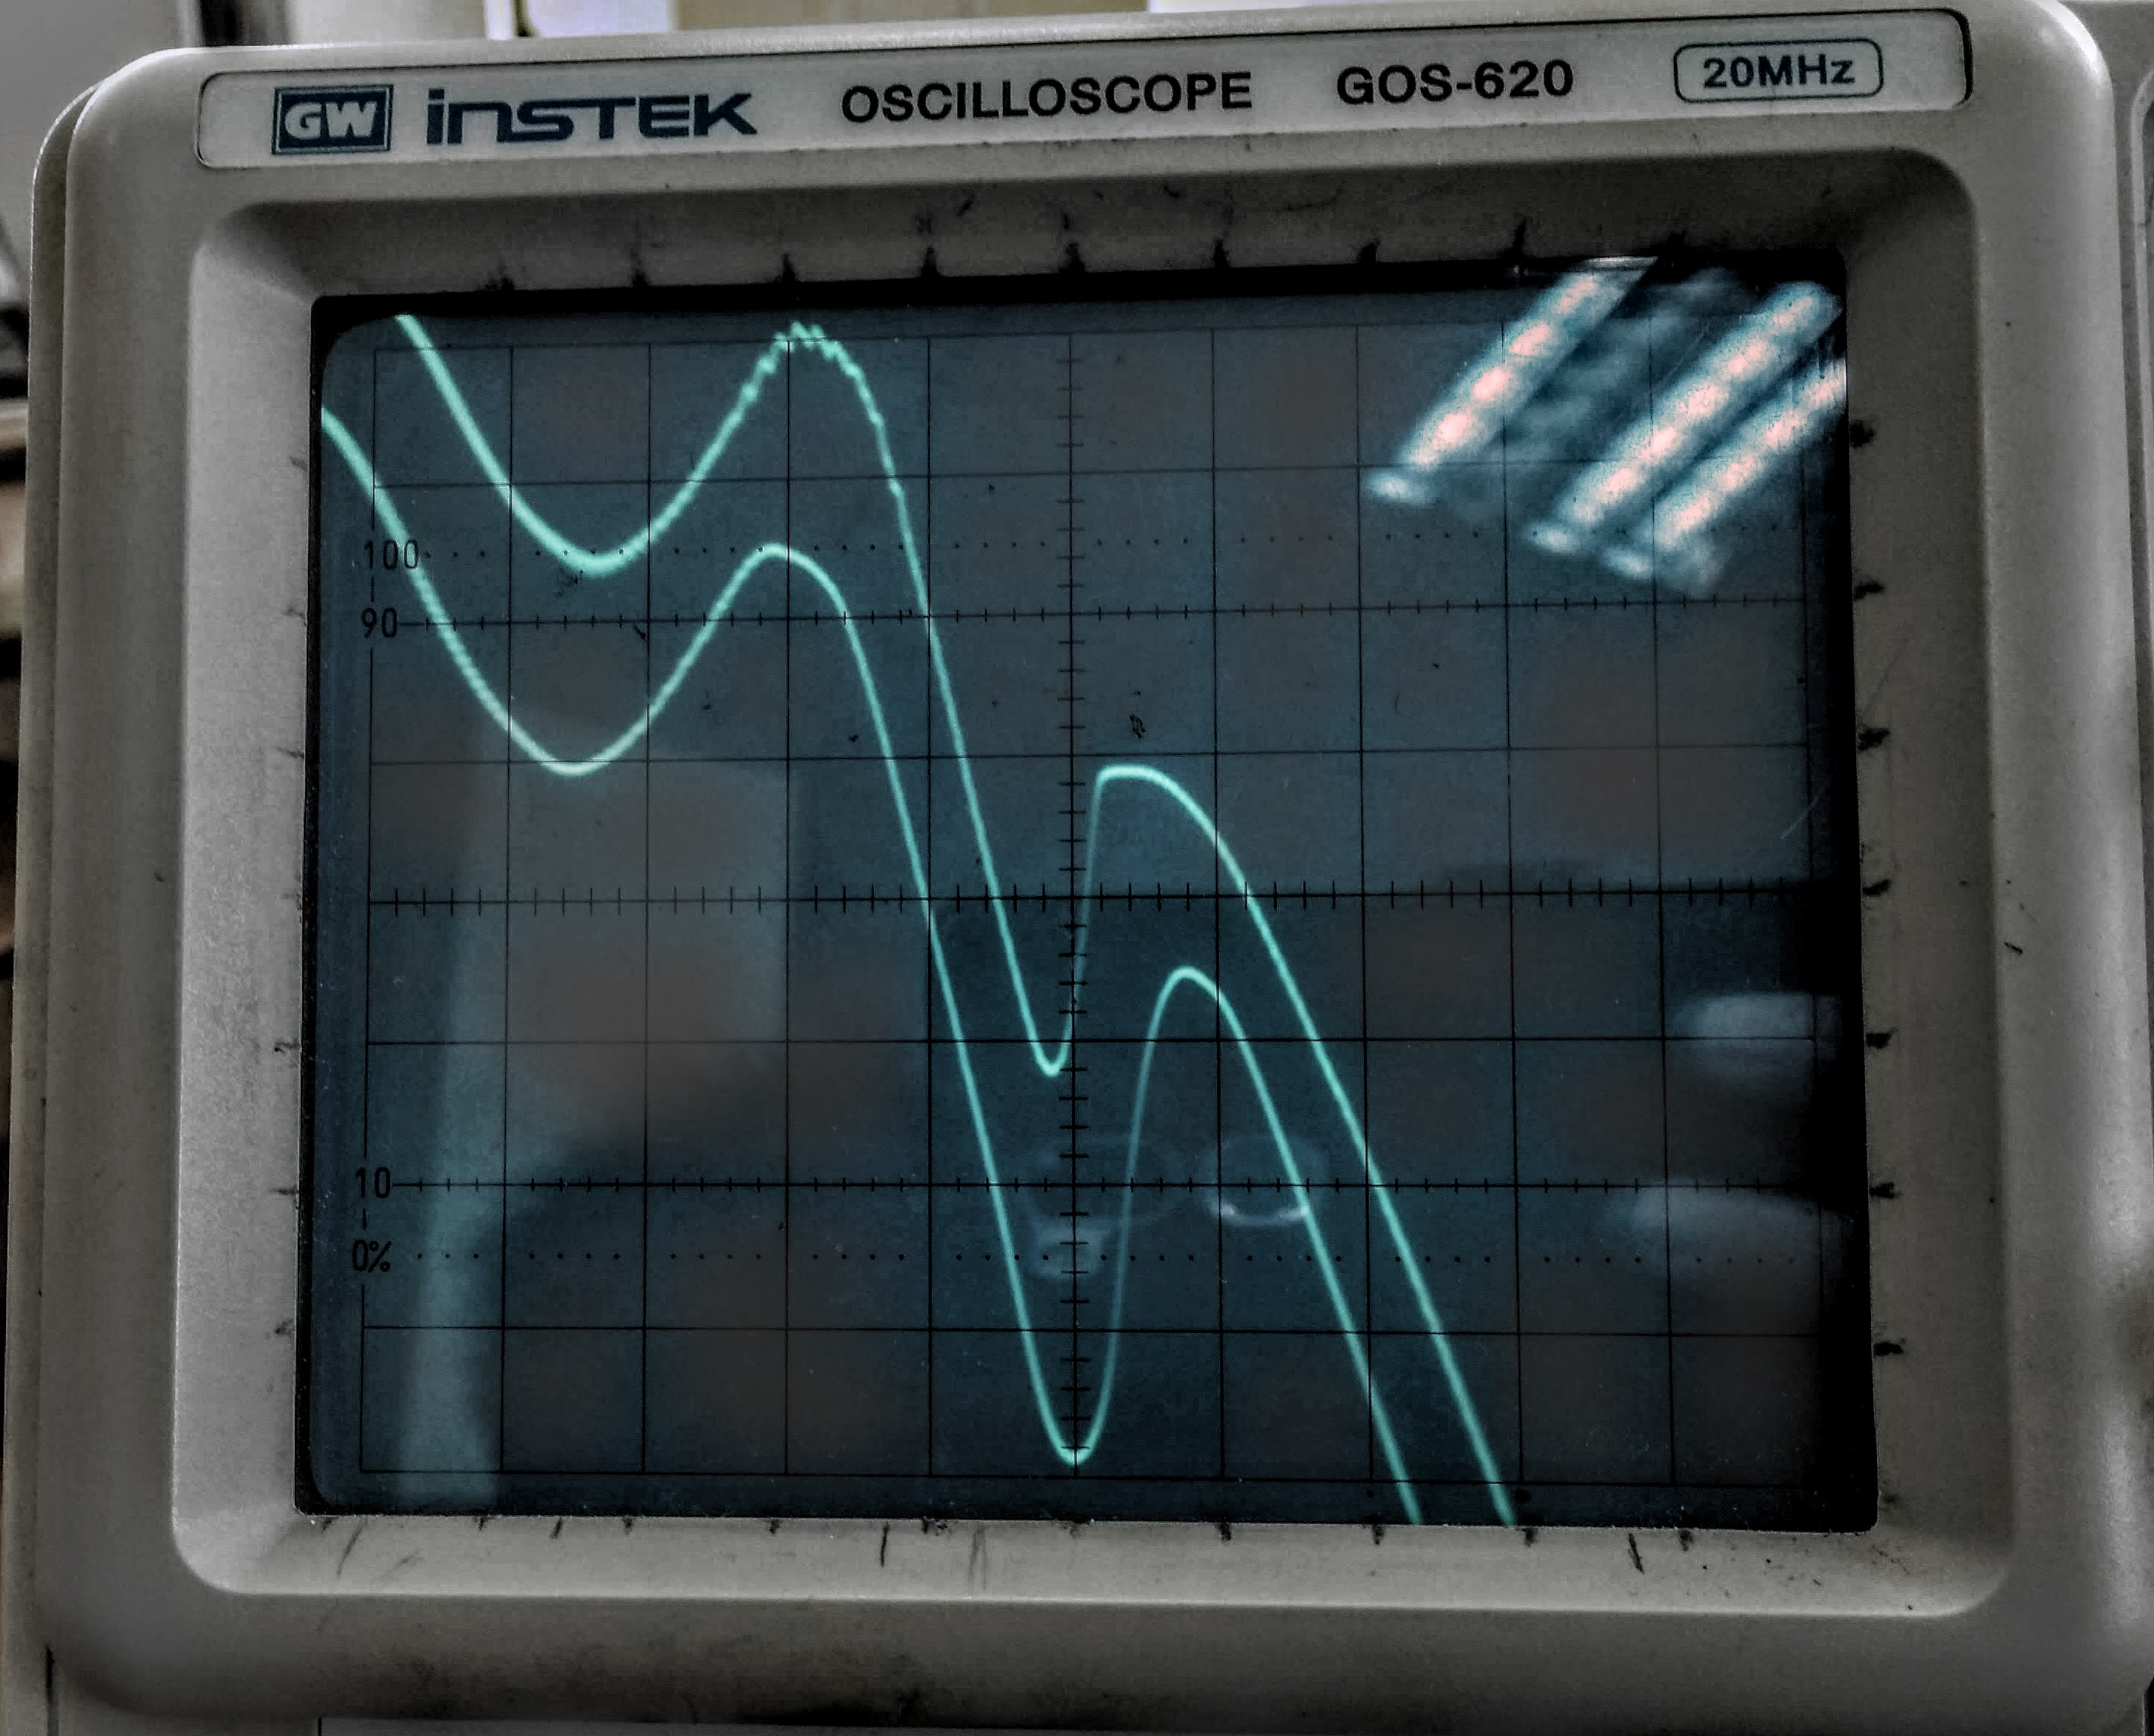
\includegraphics[width=1\linewidth]{6_V.jpg}
\caption{Осциллограмма при задерживающем напряжении 6 В}
\label{ris:experimcoded}
\end{minipage}
\hfill 
\begin{minipage}[h]{0.45\linewidth}
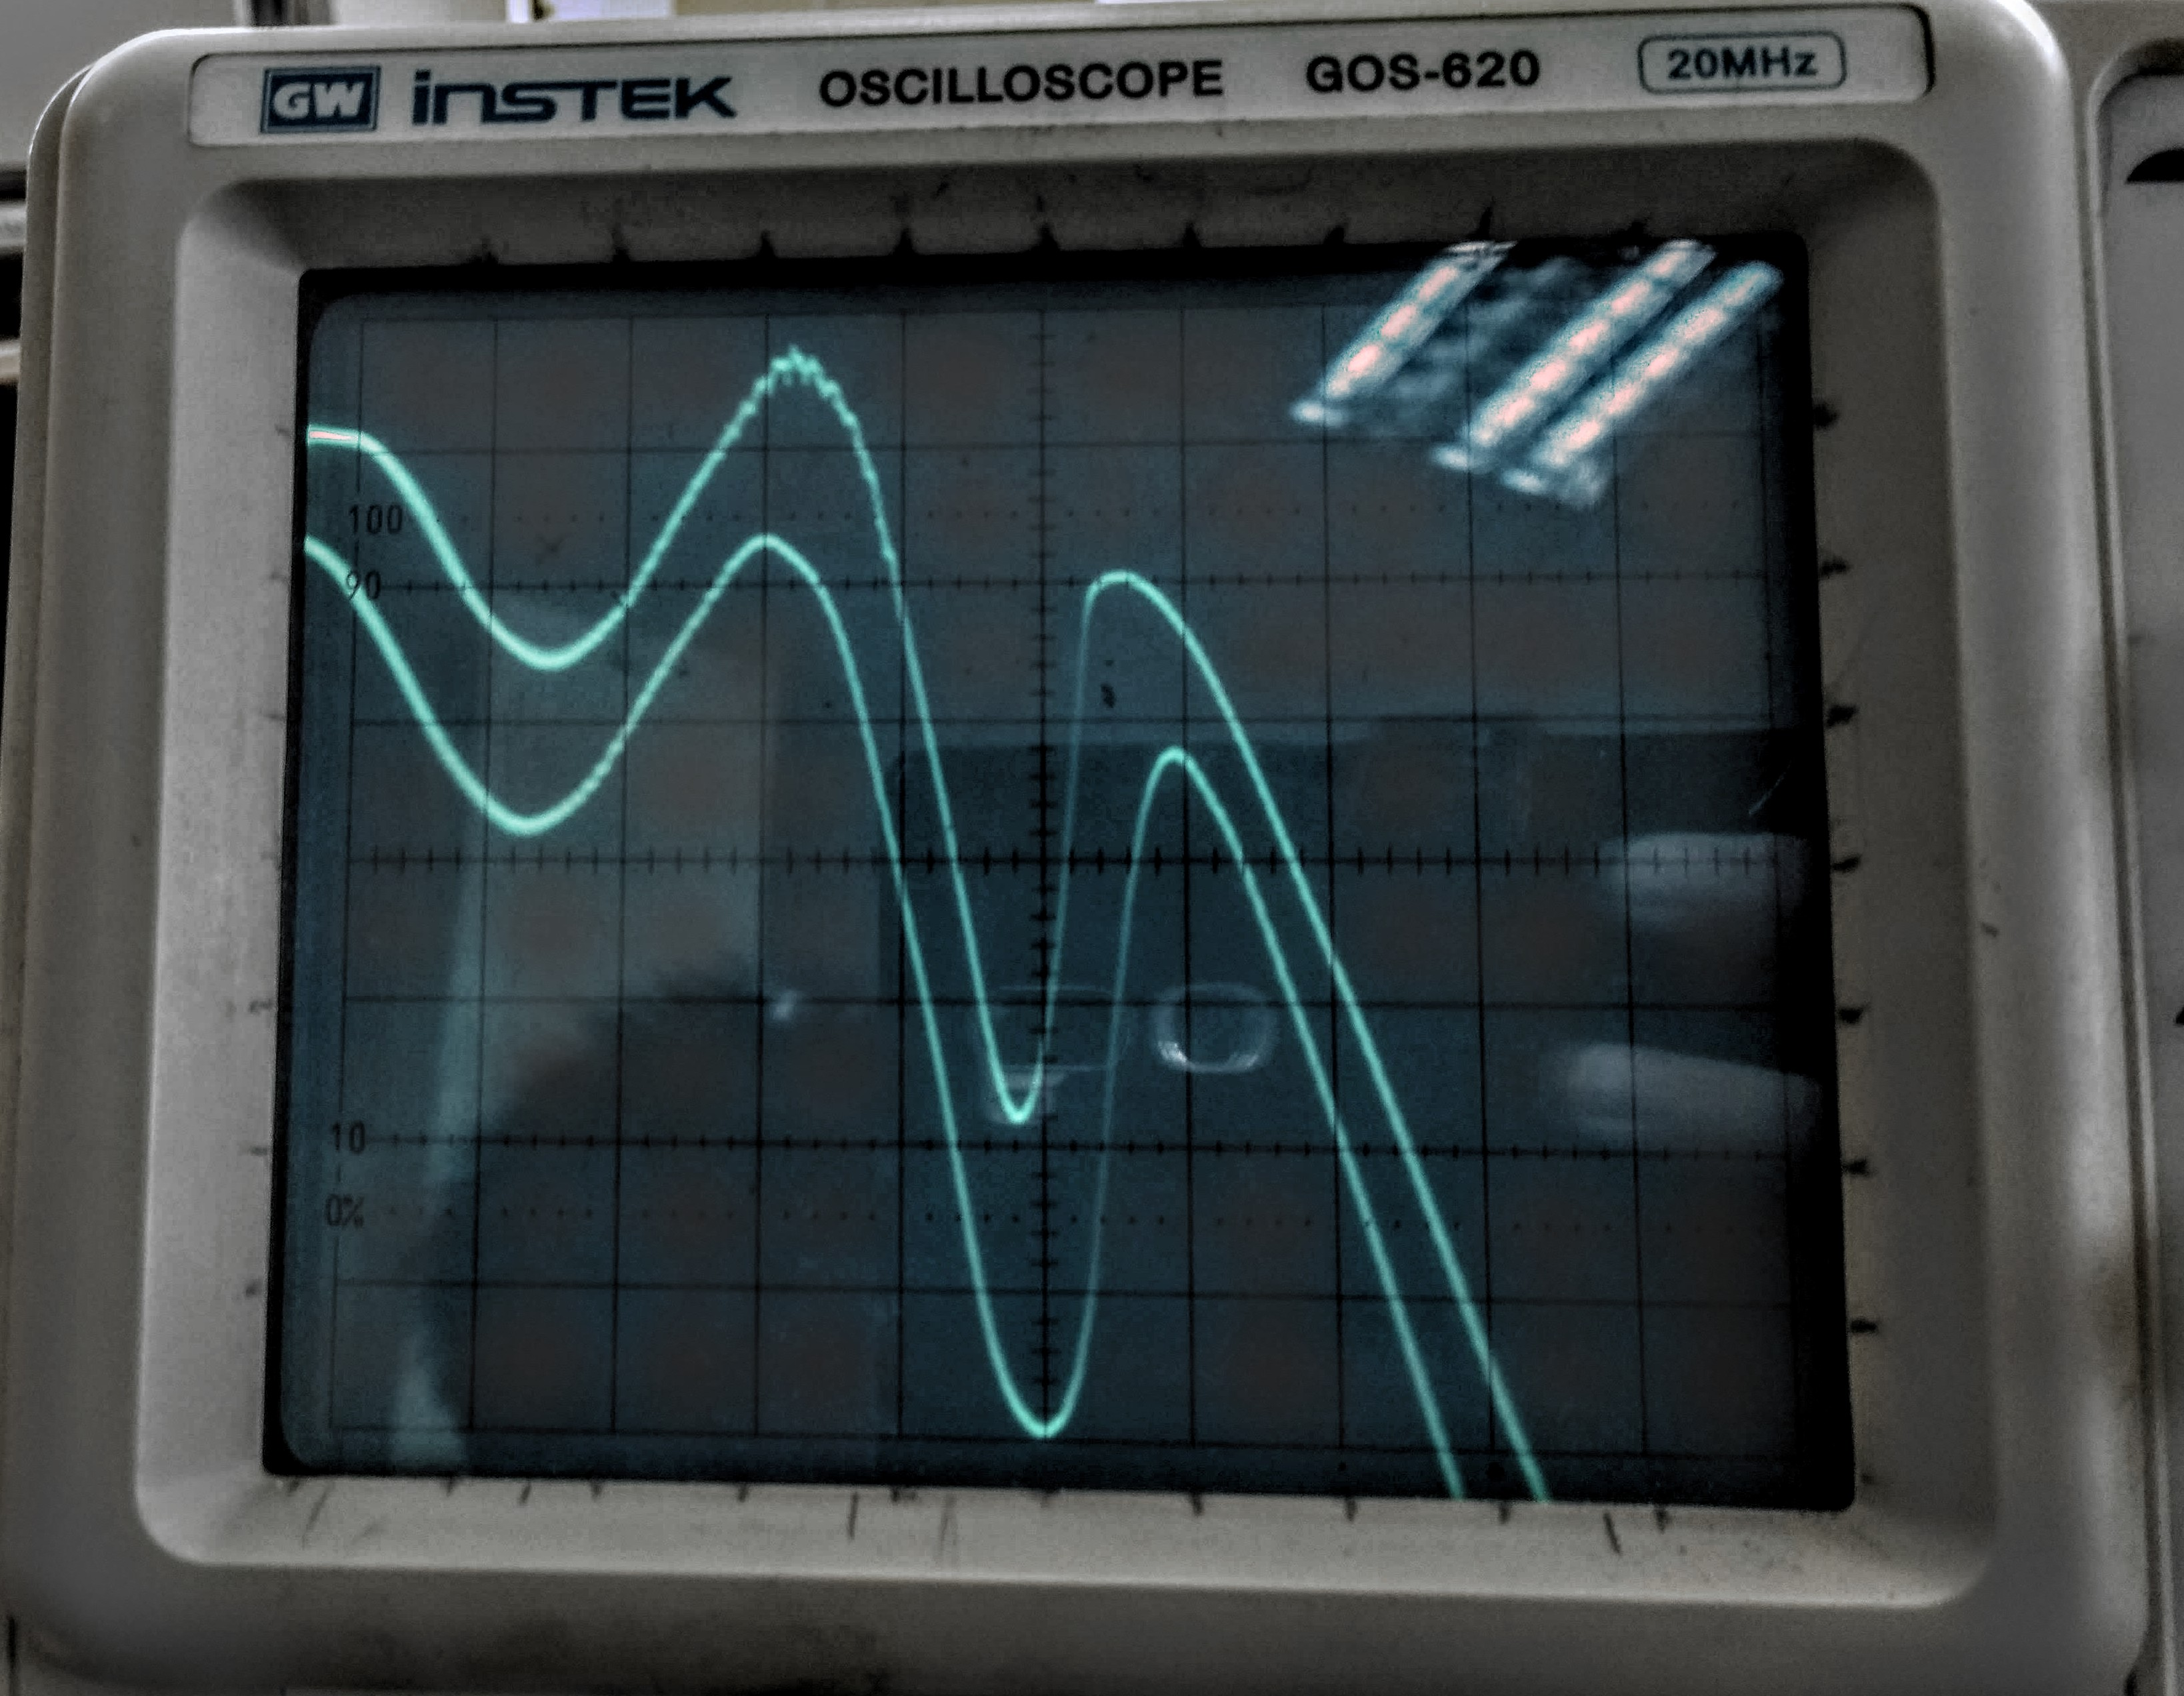
\includegraphics[width=1\linewidth]{8_V.jpg}
\caption{Осциллограмма при задерживающем напряжении 8 В}
\label{ris:experimcoded}
\end{minipage}
\end{center}
\end{figure}

\item Определим значение энергии первого возбуждённого состояния атома гелия. 
\begin{center}
    $\overline{V_{max}} = 13.7 \pm 2.5$ В \hspace{1cm} $\overline{V_{min}} = 17.5 \pm 2.5$ В
\end{center}
Погрешности определения средних значений определим, используя формулу
\begin{center}
    $\sigma_V^2_1 = \sigma_V_4^2 + \sigma_V_6^2 + \sigma_V_8^2$ - погрешность прибора \\
    $\sigma_V_2 = \sqrt{\frac{1}{6}\sum (V_i - \overline{V})}$ -  погрешность среднего значения \\
    $\sigma_V_1 = 2.5$ В \hspace{1cm} $\sigma_V_{max}_2 = 0.5 $ В  \hspace{1cm} $\sigma_V_{min}_2 = 0.4$ В
\end{center}

Среднее значение первого возбуждённого состояния атома гелия по результатам эксперимента:
\begin{center}
    $V_{exp} = 15.6 \pm 3.8$ эВ (относительная погрешность составляет 24\%)
\end{center}
При этом табличное значение данной величины составляет
\begin{center}
    $V_{th} = 21.6$ эВ
\end{center}
С учётом погрешности, экспериментальные данные близки к теоретическим.

\end{enumerate}

\subsection{Получение вольт-амперной характеристики $I_k = f(V_a)$ в статическом режиме измерений}

\begin{enumerate}
    \item Переведём переключатель режима в положение <<Статич.>>, установим максимальный ток накала
    \item Снимем зависимость коллекторного тока от анодного напряжения $I_k = f(V_a)$ для значений задерживающего напряжения 4, 6 и 8 В. Результаты измерений занесём в таблицы 2-4
    
    \begin{table}[h]
    \centering
    \begin{center}
    \caption{Значения коллекторного тока и анодного напряжения, задерживающее напряжение 4 В}
    \end{center}
    \vspace{0.1cm}
    \label{tab:my_label}
    \begin{tabular}{ |p{1cm}||p{0.6cm}|p{0.6cm}|p{0.6cm}|p{0.6cm}|p{0.6cm}|p{0.6cm}|p{0.6cm}|p{0.6cm}|p{0.6cm}|p{0.6cm}|p{0.6cm}|p{0.6cm}|p{0.6cm}|p{0.6cm}|p{0.6cm}|p{0.6cm}|p{0.6cm}|}
 \hline
$V$, В & 0.03 & 4.54 & 6.55 & 8.44 & 10.12 & 10.98 & 12.02 & 13.08 & 14.24 & 15.29 & 16.63 & 17.54 & 18.38 & 19.19 & 20.29 & 21.48 & 23.76\\
 \hline
 $I$, $\mu$А & 1 & 10 & 15 & 21 & 26 & 29 & 32 & 36 & 40 & 44 & 49 & 52 & 54 & 57 & 60 & 62 & 62\\
\hline
\hline
$V$, В & 24.47 & 25.41 & 26.72 & 28.21 & 29.52 & 30.29 & 31.8 & 33.02 & 33.7 & 34.79 & 35.94 & 37.75 & 39.26 & 41.09 & 44.21 & 49.34 & 52.32\\
\hline
$I$, $\mu$А & 62 & 53 & 56 & 61 & 67 & 72 & 75 & 81 & 86 & 89 & 92 & 93 & 94 & 93 & 89 & 86 & 90\\
\hline
 
\end{tabular}
\end{table}

    \begin{table}[h]
    \centering
    \begin{center}
    \caption{Значения коллекторного тока и анодного напряжения, задерживающее напряжение 6 В}
    \end{center}
    \vspace{0.1cm}
    \label{tab:my_label}
    \begin{tabular}{ |p{1cm}||p{0.6cm}|p{0.6cm}|p{0.6cm}|p{0.6cm}|p{0.6cm}|p{0.6cm}|p{0.6cm}|p{0.6cm}|p{0.6cm}|p{0.6cm}|p{0.6cm}|p{0.6cm}|p{0.6cm}|p{0.6cm}|p{0.6cm}|p{0.6cm}|p{0.6cm}|}
 \hline
$V$, В & 0.11 & 1.44 & 3.77 & 4.75 & 6.92 & 7.44 & 8.39 & 9.62 & 11.44 & 13.9 & 14.91 & 15.8 & 16.55 & 17.85 & 18.27 & 19.07 & 19.56\\
 \hline
 $I$, $\mu$А & 0 & 1 & 5 & 7 & 12 & 14 & 16 & 20 & 26 & 34 & 38 & 42 & 44 & 48 & 50 & 52 & 54\\
\hline
\hline
$V$, В & 19.75 & 20.38 & 21.8 & 22.54 & 23.12 & 23.82 & 24.78 & 25.4 & 27.12 & 28.3 & 31.29 & 32.43 & 33.4 & 34.16 & 35.7 & 36.68 & 39.26\\
\hline
$I$, $\mu$А & 54 & 56 & 59 & 61 & 61 & 62 & 38 & 38 & 42 & 48 & 62 & 67 & 71 & 74 & 78 & 80 & 79\\
\hline
\hline
$V$, В & 40.81 & 41.8 & 42.7 & 44.5 & 48.29 & 51.3 & 56 & 58 & 64.5 &  &  &  &  &  &  &  & \\
\hline
$I$, $\mu$А & 76 & 75 & 73 & 70 & 68 & 71 & 77 & 80 & 82 &  &  &  &  &  &  &  & \\
\hline
 
\end{tabular}
\end{table}

    \begin{table}[h]
    \centering
    \begin{center}
    \caption{Значения коллекторного тока и анодного напряжения, задерживающее напряжение 8 В}
    \end{center}
    \vspace{0.1cm}
    \label{tab:my_label}
    \begin{tabular}{ |p{1cm}||p{0.6cm}|p{0.6cm}|p{0.6cm}|p{0.6cm}|p{0.6cm}|p{0.6cm}|p{0.6cm}|p{0.6cm}|p{0.6cm}|p{0.6cm}|p{0.6cm}|p{0.6cm}|p{0.6cm}|p{0.6cm}|p{0.6cm}|p{0.6cm}|p{0.6cm}|}
 \hline
$V$, В & 3 & 9.29 & 12.27 & 15.23 & 16.7 & 17.42 & 18.23 & 19.43 & 21.72 & 23.09 & 24.1 & 24.8 & 25.33 & 25.62 & 27.11 & 28.7 & 29.8\\
 \hline
 $I$, $\mu$А & 0 & 9 & 24 & 34 & 40 & 42 & 45 & 49 & 55 & 58 & 59 & 60 & 60 & 25 & 25 & 30 & 36\\
\hline
\hline
$V$, В & 31.12 & 34.46 & 37.03 & 38.75 & 39.22 & 40.02 & 40.76 & 42.08 & 43.6 & 45.5 & 46.75 & 50.4 & 52.2 & 54.4 & 61.6 & 64.32 & \\
\hline
$I$, $\mu$А & 43 & 59 & 64 & 66 & 65 & 64 & 62 & 60 & 57 & 53 & 51 & 50 & 51 & 53 & 59 & 59 & \\
\hline
 
\end{tabular}
\end{table}

\item Представим графики вольт-амперных характеристик трёхэлектродной лампы при разных задерживающих напряжениях на рис. 7

\begin{figure}[h]
    \centering
    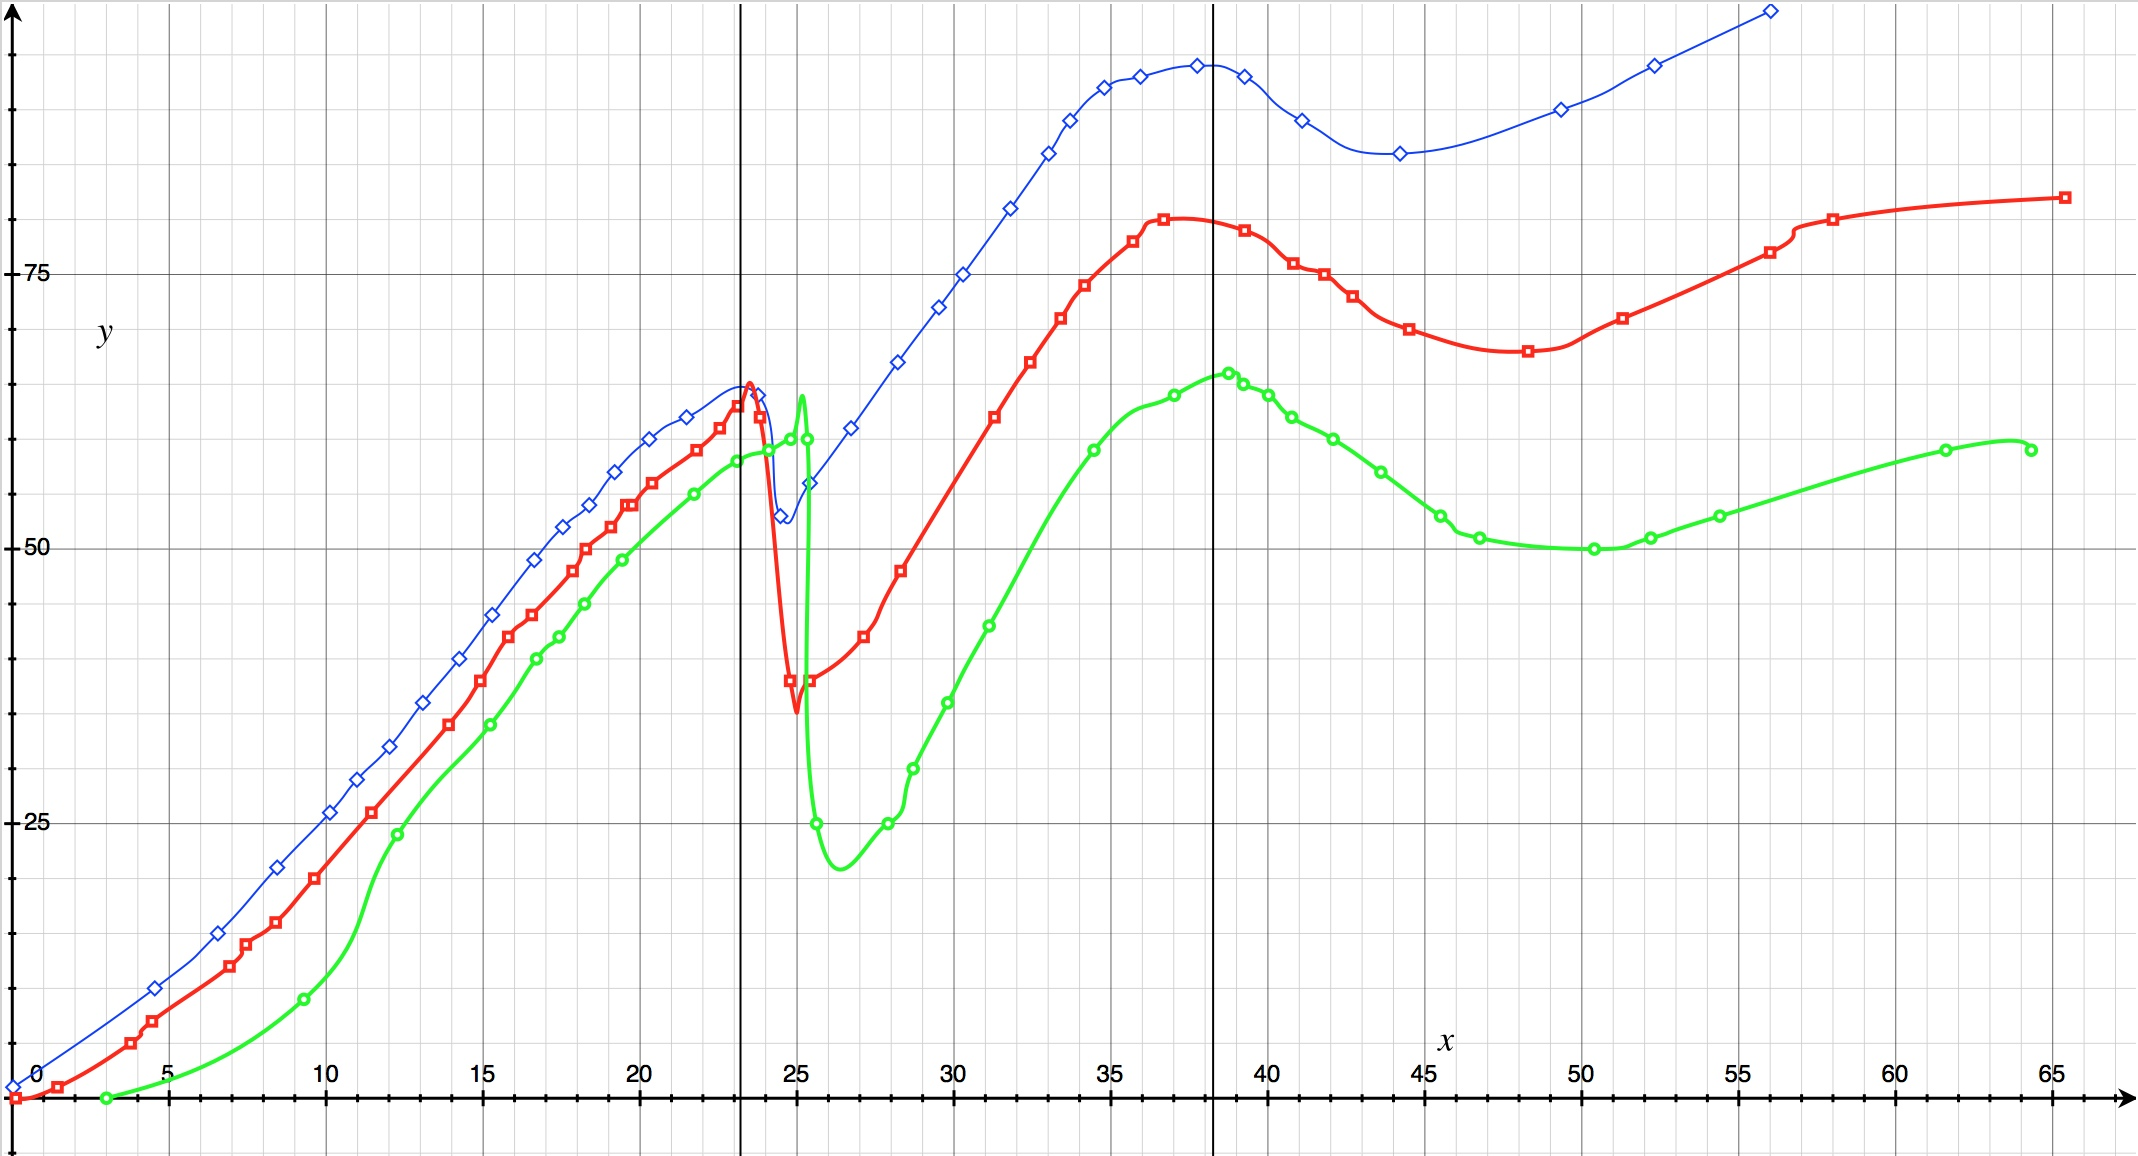
\includegraphics[width=\textwidth]{fig2.jpg}
    \caption{Вольт-амперные характеристики трёхэлектродной вакуумной лампы при разных значениях запирающего напряжения}
    \label{fig:vac}
\end{figure}

\item Определим по результатам измерений энергию первого возбуждения атома гелия. Воспользуемся принципом, описанным в 5.1. и занесём максимальные и минимальные значения напряжения в таблицу 5.

\begin{table}[h]
    \centering
    \begin{center}
    \caption{Максимумы и минимумы напряжения на осциллограммах}
    \end{center}
    \vspace{0.1cm}
    \label{tab:my_label}
    \begin{tabular}{ |p{3.5cm}||p{1.5cm}|p{1.5cm}|p{1.5cm}|p{1.5cm}|p{2.5cm}|p{1.5cm}|p{1.5cm}|}
 \hline
Задерж. напряжение & $V_{max_1}$ & $V_{max_2}$ & $V_{min_1}$ & $V_{min_2}$ & Погрешность & \triangle V_{max} & \triangle V_{min}\\
 \hline
 4 В & 23.76 В & 39.26 В & 25.41 В & 49.34 В & 1 В & 15.5 В & 23.93 В\\
\hline
 6 В & 23.82 В & 36.68 В & 24.78 В & 48.29 В & 1 В & 12.86 В & 23.51 В\\
\hline
 8 В & 25.33 В & 38.75 В & 25.62 В & 50.40 В & 1 В & 13.42 В & 24.78 В\\
\hline

\end{tabular}
\end{table} 

\item Определим значение потенциала возбуждения атома гелия, оно соответствует расстоянию между экстремумами одного типа
\begin{center}
    $\overline{V_{max}} = 14.93 \pm 1.92$ В \hspace{1cm} $\overline{V_{min}} = 24.07 \pm 1.80$ В
\end{center}
Погрешности определения средних значений определим, используя формулу
\begin{center}
    $\sigma_V^2_1 = \sigma_V_4^2 + \sigma_V_6^2 + \sigma_V_8^2$ - погрешность прибора \\
    $\sigma_V_2 = \sqrt{\frac{1}{6}\sum (V_i - \overline{V})}$ -  погрешность среднего значения \\
    $\sigma_V_1 = 1.73$ В \hspace{1cm} $\sigma_V_{max}_2 = 0.83 $ В  \hspace{1cm} $\sigma_V_{min}_2 = 0.48$ В
\end{center}

Среднее значение первого возбуждённого состояния атома гелия по результатам эксперимента:
\begin{center}
    $V_{exp} = 19.5 \pm 3.42$ эВ (относительная погрешность составляет 18\%)
\end{center}
При этом табличное значение данной величины составляет
\begin{center}
    $V_{th} = 21.6$ эВ
\end{center}
С учётом погрешности, экспериментальные данные близки к теоретическим.

\end{enumerate}    

\newpage

\section{Вывод}

В ходе работы был воспроизведён опыт Франка-Герца, подтверждающий наличие дискретных уровней возбуждения атомов. Вольт-амперная характеристика трёхэлектродной вакуумной лампы была измерена двумя способами - динамическим и статическим. По этим ВАХ были экспериментально определены потенциалы возбуждения атомов гелия (одноатомный газ, заполняющий лампу). 
\begin{center}
    $V_{exp}_d = 15.6 \pm 3.8$  эВ \\
    $V_{exp}_s = 19.5 \pm 3.42$ эВ \\
    $V_{th} = 21.6 $ эВ
\end{center}
Видим, что результаты совпадают по порядку величины, также значение потенциала возбуждения атома гелия в пределах погрешности совпадает с табличным значением. Статический метод оказался более точным, чем динамический. \par
Стоит отметить, что при наличии более совершенной установки можно выполнить более точные измерения ВАХ, тем самым определив потенциалы возбуждения других дискретных уровней, а также потенциалы ионизации.

\end{document}
